
%%%%%%%%%%%%%%%%%%%%%%%%%%%%%%%%%%%%%%%%%%%%%
\section{Quick sort의 캐시 히트율}

\begin{figure}[h!]
    \centering
    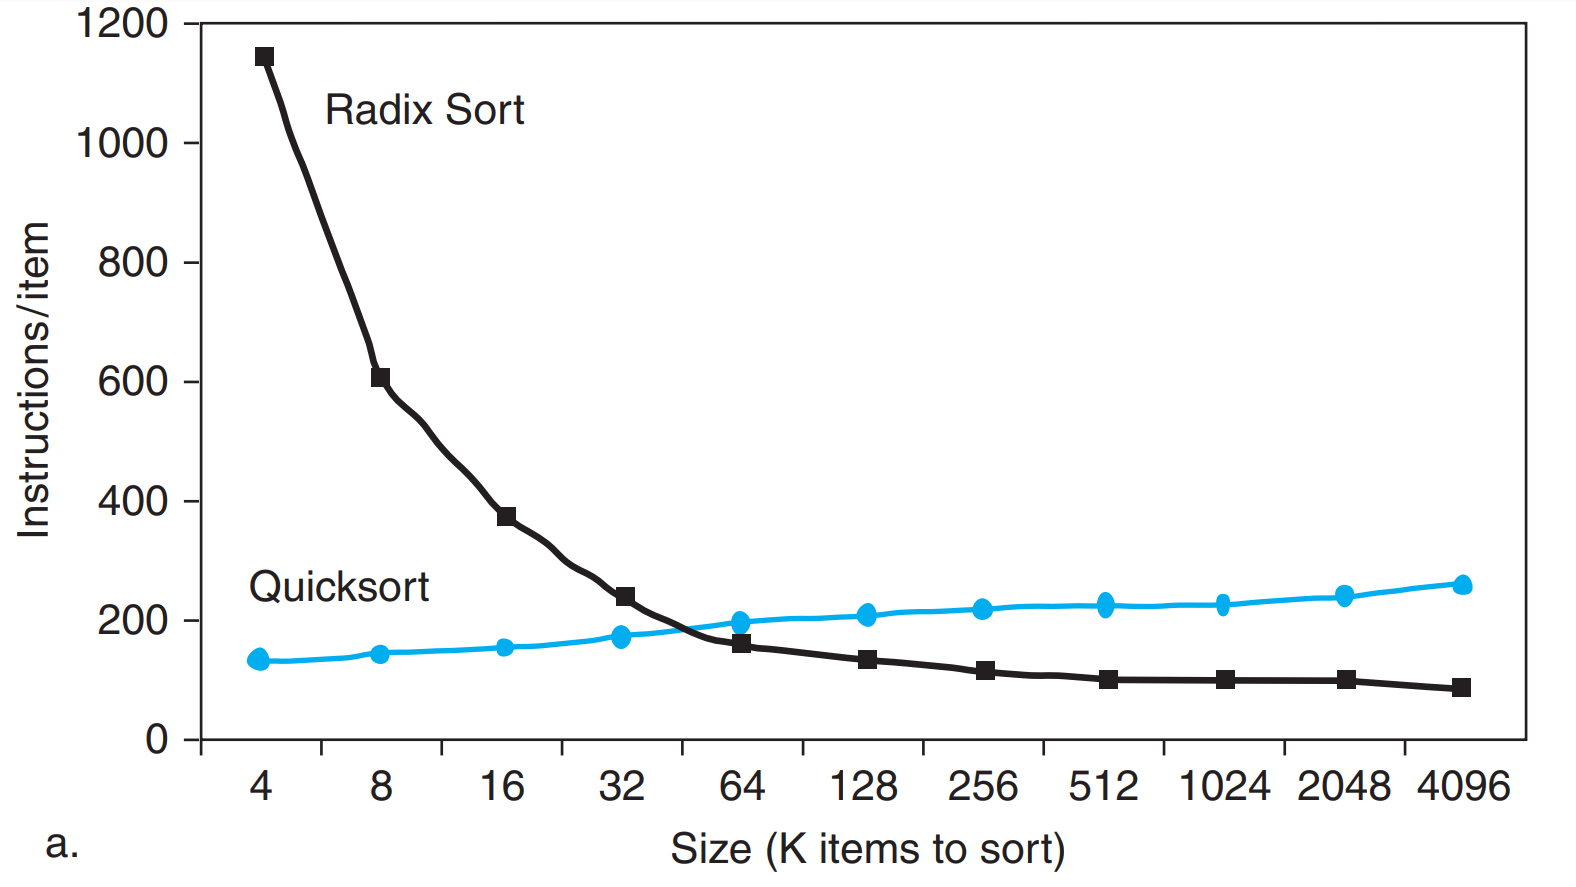
\includegraphics[scale=0.3]{{QuickSort/pic/quick1.png}}
\end{figure}

다음은 Radix sort(기수 정렬)과 Quick sort의 입력 n에 따른 수행 명령어 수/n를 나타낸 것이다. 
기수 정렬의 시간복잡도는 $O(n)$이나 최고차항의 계수가 커서 초반 입력 n에 대해서는 Quick sort가 빠른 것을 보여준다.

그러나 실제 수행시간과 캐시 미스율를 비교해 봤을때, 퀵소트가 높은 캐시 적중률로인해 기수정렬보다 약간 더 빠름을 볼 수 있다.
이는 알고리즘적인 부분만으로는 알수없는 결과기에 실제 컴퓨터 구조의 캐시 개념을 알아야한다.
작성자 의견: 해당 그래프에서 n의 수치가 최대가 5000으로 나와있는걸 생각해볼때 값이 정말 커지면 결국에는 시간복잡도에 따라 기수정렬이 더 빠름이 명확할것으로 예상한다.


\newpage

\begin{figure}[h!]
    \centering
    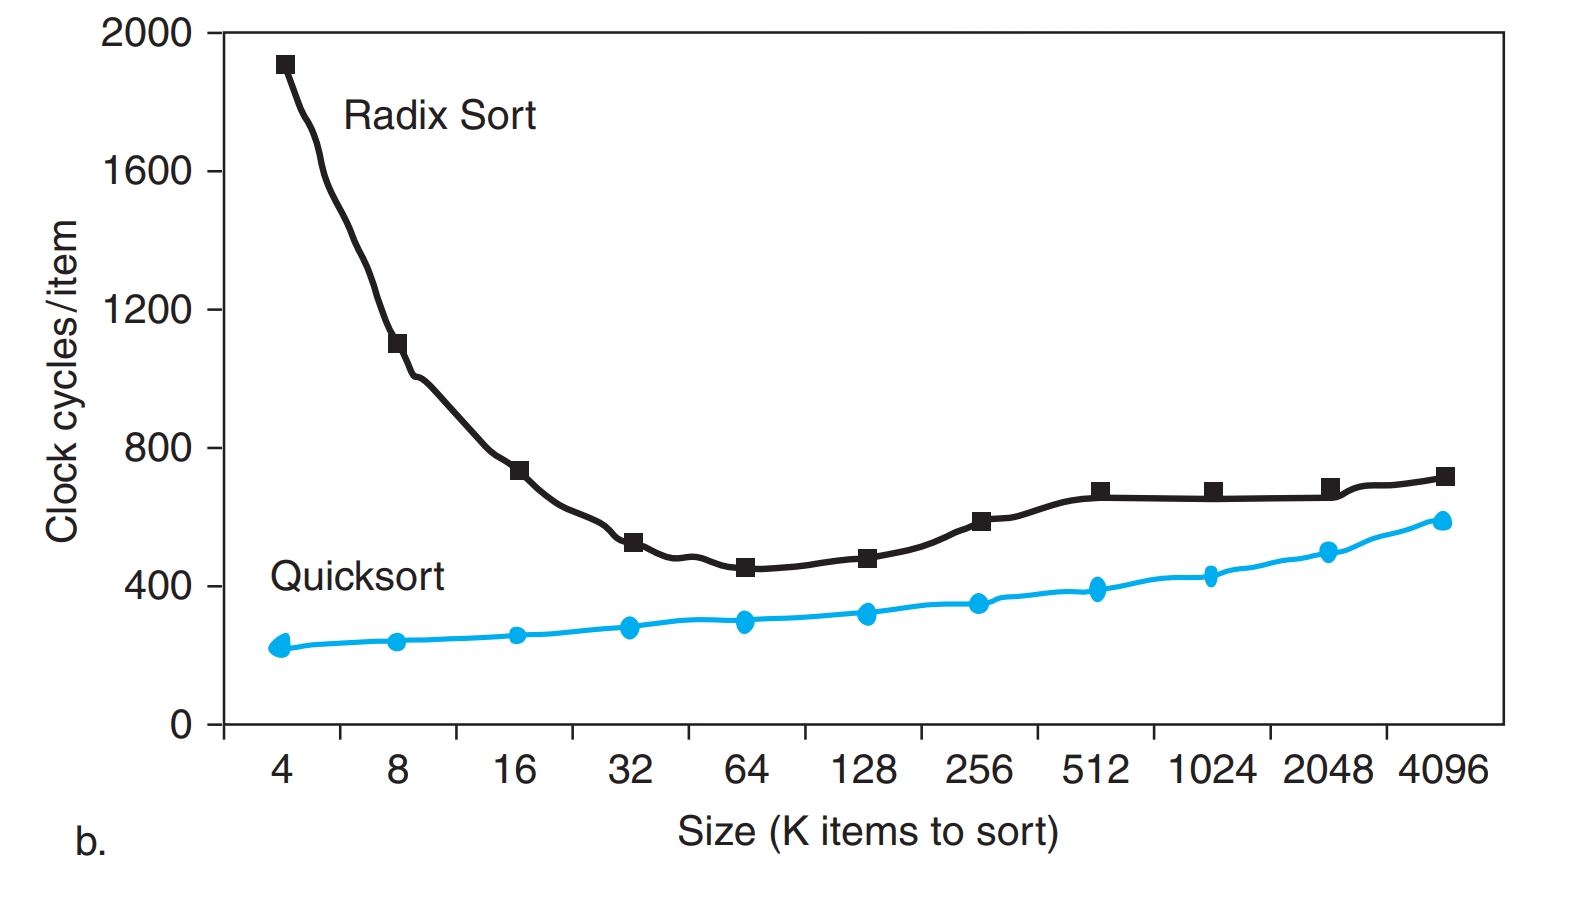
\includegraphics[scale=0.3]{{QuickSort/pic/quick2.png}}
    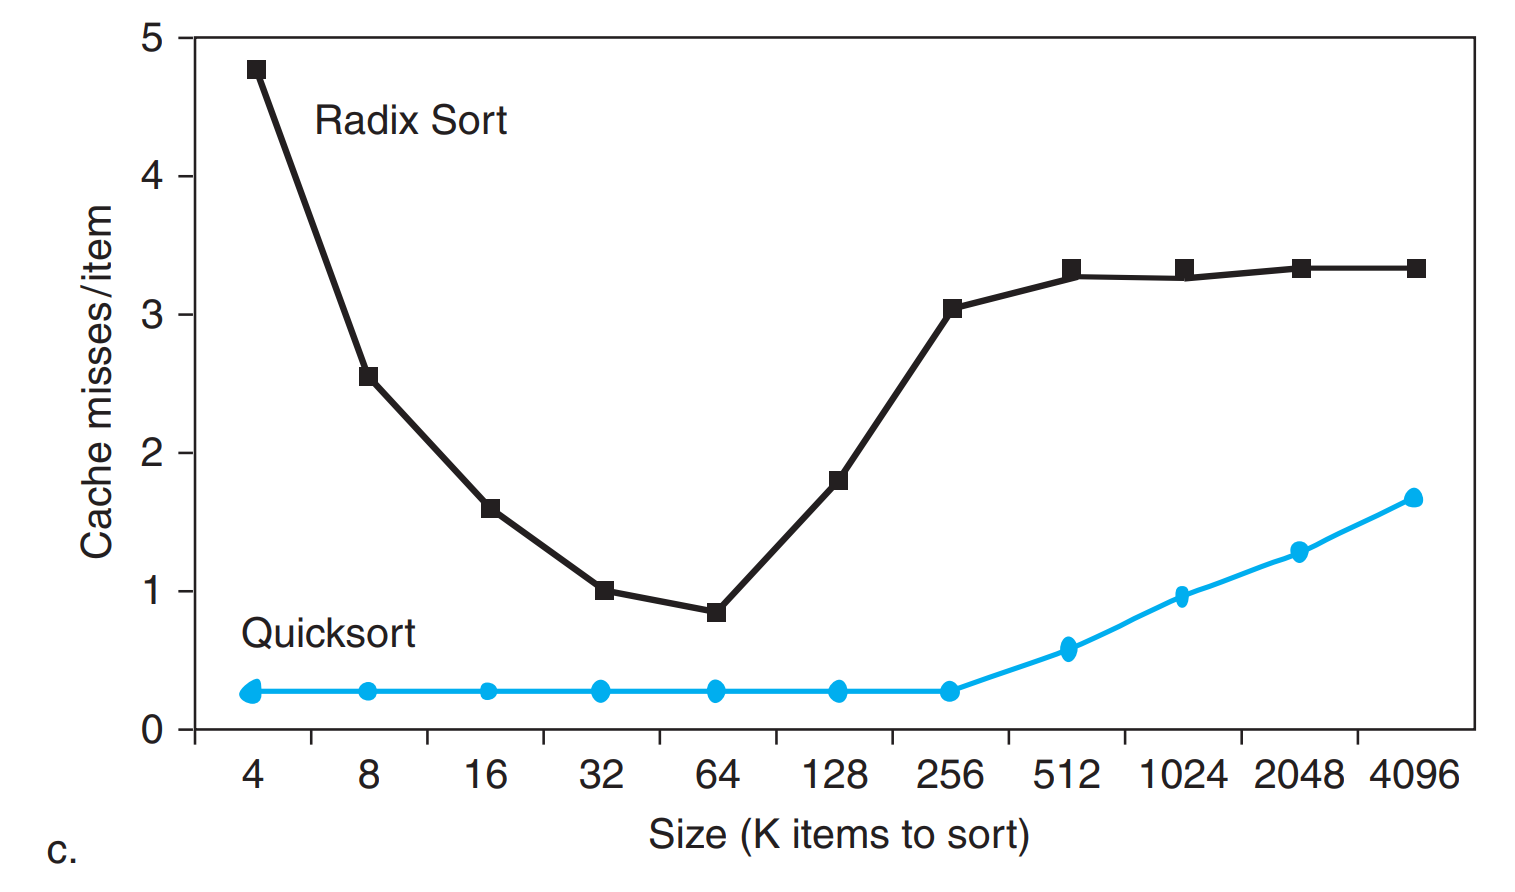
\includegraphics[scale=0.3]{{QuickSort/pic/quick3.png}}
    \caption{Comparing Quicksort and Radix Sort by (a) instructions executed per item sorted (b) time per item sorted, and (c) cache misses per item sorted. This data is from a paper by LaMarca and Ladner [1996]. Due to such results, new versions of Radix Sort have been invented that take memory hierarchy into account, to regain its algorithmic advantages. Th e basic idea of cache optimizations is to use all the data in a block repeatedly before it is replaced on a miss.\cite{reference2}}
\end{figure}

\newpage
%%%%%%%%%%%%%%%%%%%%%%%%%%%%%%%%%%%%%%%%%%%%%%%%%%%%%%%%%%%%%%%%%%%%%%%%%%%%
